\chapter{Introduction}
\label{chap:intro}
Information extraction (IE) from the web pages is a popular task, and the goal of IE is the automatic extraction of structural data from unstructured or semi-structured one. Web Extraction (WE) is a particular case of IE where the corpus of documents is a webpages. In the thesis, we are solving the problem of WE for the specific types of the data, namely the Social Event extraction from a webpage.   


% In the general case, IE algorithm should \textit{learn} how to extract the meaningful structural information from the training labeled data and then be able to do the same on previously unseen data with reasonable quality. This formulation allows considering IE problem as a machine learning task.\\



\section{Motivation}
Besides the obvious application of WE in the search engine, there are also so-called vertical web services where WE is widely used too. Such websites allow to explore and work with the information on a specific topic. Such services usually do not produce the content by themselves, and rather they automatically collect the data from various sources, processes this data in some way and present to the user in the appealing form. Such services also called \textit{aggregators}. A broad list of topics includes news, retail and other advertisements, reviews, flight tickets, videos and pictures, recipes, social networks and many other. The list is very extensive, virtually for any topic discussed and presented on the Internet there are aggregators exist which try to grasp all other sources into one. \\

Aggregators are usually very popular because they provide the user with the big database, rich functionality, flexibility and instant updates, what helps a user to save time. Due to popularity of aggregator the 'original' content maker is becoming popular too and therefore the content maker has resources to produce new interesting content. The other side of this practice is traffic reduction on the original content maker websites. It happens for example if the aggregator is unfair and doesn't show the source of information. \\

The relationship between aggregators and original source makers today reminds the problem of chicken and egg. That's why search engines are very accurate with automatic extraction at the moment of showing the result for the search query. If Google shows you the correct answer right when you type the question, the website with this particular answer where Google took the information from will lose the user. Since this site loses the user, it also loses monetizing and resources to produce the 'correct answers' in future; hence Google will lose the sources of correct answers. That's the reason why IE among Internet industry players is a controversial topic.\\

In the research area, IE of web pages is typically used in the tasks related to natural language processing and text mining. The reason for this is that the web page content is the semi-structured text mixed with the HTML markdown. Many research project centered around the analysis of various news sources as news articles, tweets, social networks, etc. Some of the possible tasks are sentiment analysis of news, topic recognition, summarization. Some projects aim to build the system which determines the answer on human-language question based on huge amount of processed text as IBM Watson \cite{IBMAlchemy} or Wolfram Language \cite{Wolfram}.\\      

The extraction of data from the web page is usually linked with the Document Object Model (DOM) processing and implies the understanding of the web page structure from the 'browser' point of view. \\

In this way, IE is becoming a quite interesting, actual and challenging task. It includes both the technical background for the data retrieving and manipulation as well as theoretical background for the reasonable model building. This thesis includes all necessary parts of this task.

\section{Problem definition}
In the thesis, we aim to create the system which automatically extracts the \textit{event components} of the social events from the web page. The social events might include musical concerts, meetings, performances, festivals, cinema and other social activities. Such events may be published on the different websites, usually on a website of the event organizer.\\

To classify the entity on a web page as an event let's state that it must have the following \textit{event components}:
\begin{enumerate}
    \item The title
    \item The description
    \item The date and time
    \item Certain location where event is taking place
\end{enumerate}

In this thesis, we won't solve the problem of identifying if the event announcement is placed on the web page since it is the task from Information Retrieval field. We assume that the page already has an event and we want to find and extract the structured information about it (i.e. extract four items above). On the picture \nameref{fig:webevent} you can see an ordinary example of the page where four main event components are circled in red.\\

We consider \textit{the webpage} as the rendered page where primary JavaScript already executed (it may be executed in future if the user interacts with a page). Such page has several important components: DOM tree, corresponding CSS, HTML code, resources (e.g. images) and rendered picture which the browser displays us. \\

For a webpage, we will collect all web elements from a DOM tree, and four of them would be components we need to extract. We will collect more than two hundreds features for every web element and build the model which distinguishes an event components from all other elements. In our problem we will consider four one-vs-all classifiers where each of them will refer and detects corresponding event component. 

\begin{figure}[h]
\begin{center}
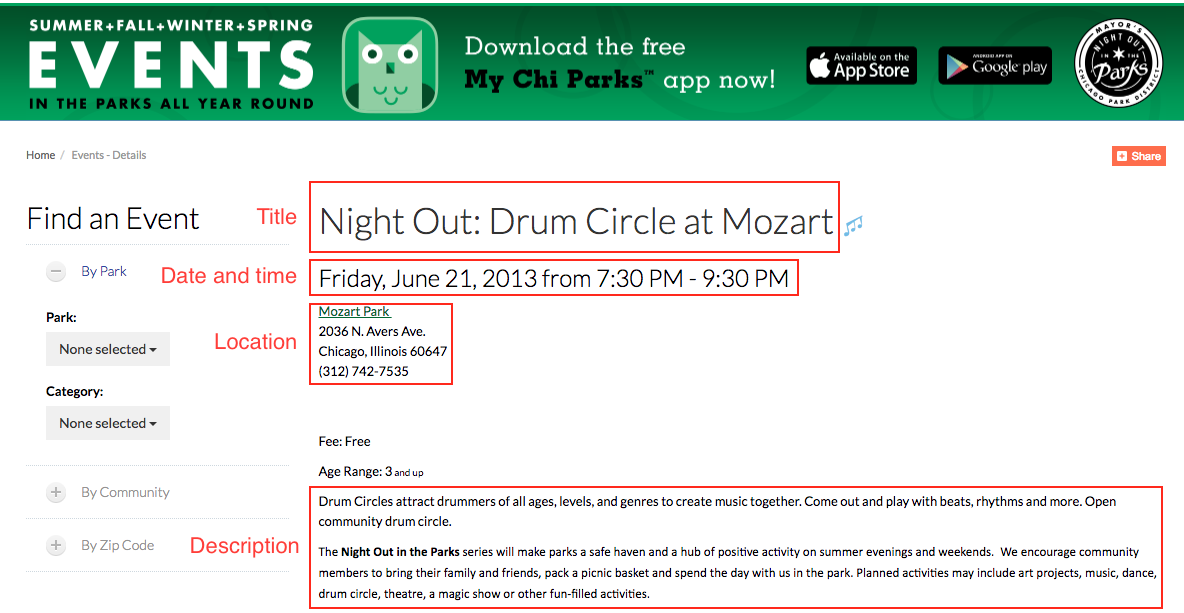
\includegraphics[height=7cm]{figures01/event_example}
\caption{An example of the social event on a webpage}
\label{fig:webevent}
\end{center}
\end{figure}


\section{Thesis Outline}
The thesis consists of 8 chapters, \nameref{chap:conclusion}, \nameref{append} and \nameref{chap:cd}. The current chapter briefly describes the idea of the thesis and motivation for the task of web extraction. Chapter \ref{chap:background} covers necessary considers important web concepts for this work (webpage, DOM, XPath, Microdata semantic markup, etc.). Chapter \ref{chap:webextr} refers to an overview of state of the art Web Extraction techniques and related work. In chapter \ref{chap:design} we explain the structure of Sociopath system together with the description of its main components. The method which we propose for the collecting of the training dataset will be discussed in details in chapter \ref{chap:datacollect}. Last three chapters are devoted to a cyclic technical process of the dataset analysis. In chapter \ref{chap:clean} we will do several cleaning procedures in order to make the dataset reliable. In \ref{chap:dataexplore} we show the visualization and precise analysis of the extracted features and its relationships. In \ref{chap:model} we will build  and evaluate several classification models. \nameref{chap:conclusion} will sum up our most valuable contributions and propose ideas for further work.